\chapter{The Eagle Squad}
\label{chap:squad}

You will fly missions for the Eagle Squad, which
is known for a good equipment and the best pilots.
Just look at the fighter and pilot overviews.


\section{The Fighters}
\label{sec:fighters}

\begin{center}
\begin{tabular}{|c|l|}
\hline
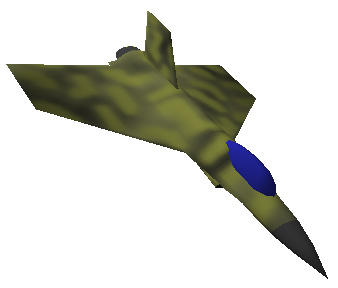
\includegraphics[width=4cm]{falcon.jpg} &
The GL-16 Falcon is an advanced fighter of the Eagle squadron.\\
\hline
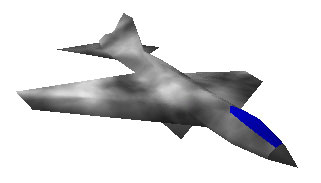
\includegraphics[width=4cm]{crow.jpg} &
The Crow is a typical enemy fighter.\\
\hline
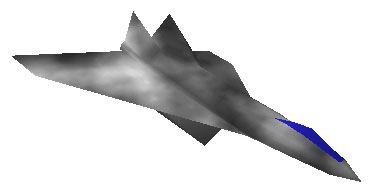
\includegraphics[width=4cm]{hawk.jpg} &
The GL-22 Hawk is the Red Eagle's bomber.\\
\hline
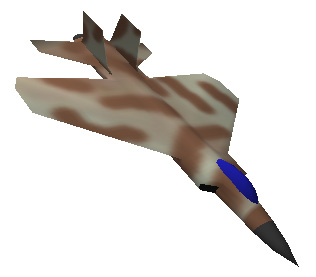
\includegraphics[width=4cm]{swallow.jpg} &
The Swallow is an advanced enemy bomber.\\
\hline
\end{tabular}
\end{center}


\section{The Weapons}
\label{sec:weapons}

\begin{center}
\begin{tabular}{|c|l|}
\hline
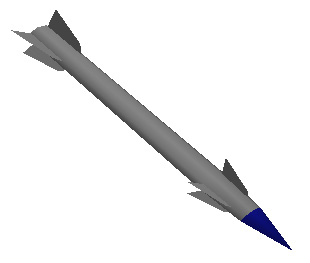
\includegraphics[width=3cm]{missile_ff.jpg} &
The FF is a radar controlled friend-foe air-air missile.\\
\hline
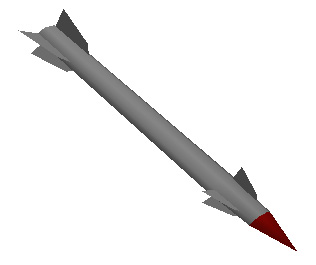
\includegraphics[width=3cm]{missile_ir.jpg} &
The IR is an infra red air-air missile.\\
\hline
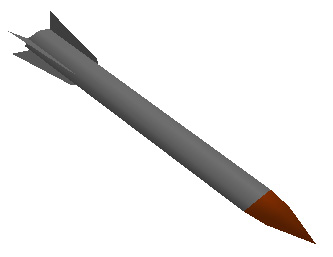
\includegraphics[width=3cm]{missile_agm.jpg} &
The AGM is a medium air-ground missile.\\
\hline
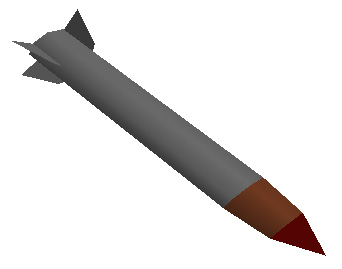
\includegraphics[width=3cm]{missile_df.jpg} &
The DF is an uncontrolled dumb fire missile.\\
\hline
\end{tabular}
\end{center}

Use FF missiles early when approaching the enemy.
They will search their target using a radar system,
however a chaff cloud may fool them.

IR missiles can only track the enemy by heat and must
therefore be fired at the enemy's back.
Flares consisting of burning magnesium can be used as a countermeasure.

AGMs are radar controlled missiles used to
take out medium ground targets like tanks.

DF missiles will only fly straight ahead like cannon shots,
but can cause an enormous amount of damage,
so they are used to take out huge ground targets like buildings.
